\documentclass[twocolumn]{article}

% General physics constructs
\newcommand{\bra}[1]{\langle #1 |}
\newcommand{\ket}[1]{| #1 \rangle }
\newcommand{\braket}[2]{\langle #1|#2\rangle}
\newcommand{\bbraket}[3]{ \langle #1 | #2 | #3 \rangle }
\newcommand{\boltzmann}{k_b}

% Common math
\newcommand{\norm}[1]{\left \lvert #1 \right \rvert}
\newcommand{\abs}[1]{\left \lvert #1 \right \rvert}  % These two are redundant. Consider removing one.

\newcommand{\avg}[1]{\left \langle #1 \right \rangle}  % Should get rid of this, as "average" isn't specific.
\newcommand{\angavg}[1]{\left \langle #1 \right \rangle}

\newcommand{\VS}{\textit{\textbf{V}}}
\newcommand{\Tr}{\textrm{Tr}}
\renewcommand{\Re}{\textrm{Re}}
\renewcommand{\Im}{\textrm{Im}}
\newcommand{\basis}[1]{\{\ket{#1}\}}

% Quantum
\newcommand{\nboseeinstein}{n_\text{BE}}
\newcommand{\gammaup}{\Gamma_\uparrow}
\newcommand{\gammadown}{\Gamma_\downarrow}
\newcommand{\gammaupdown}{\Gamma_{\uparrow \downarrow}}
\newcommand{\gammaemission}{\Gamma_\text{loss}}
\newcommand{\qualityfactoremission}{Q_{d,\text{loss}}}

% Qubits
\newcommand{\omegaqubit}{\omega_{10}}

% Circuits
\newcommand{\impedance}{Z_0}
\newcommand{\resistorsource}{R_s}
\newcommand{\vsource}{V_s}
\newcommand{\vsourcerms}{V_{s,\text{rms}}}
\newcommand{\vloadrms}{V_{l,\text{rms}}}

% Signals and noise
\newcommand{\psdsingle}{S_\text{ss}}
\newcommand{\psddouble}{S_\text{ds}}
\newcommand{\noiseavailable}{S_{p,a}^e}
\newcommand{\spectralengineer}{S^e}
\newcommand{\spectralsymmetric}{S^\text{symm}}
\newcommand{\spectralattenuator}{\spectralengineer_{\poweravailable, \text{att.}}}

% Microwaves
\newcommand{\vright}{V_+}
\newcommand{\vleft}{V_-}
\newcommand{\iright}{I_+}
\newcommand{\ileft}{I_-}
\newcommand{\poweravailable}{P_a}

% Figures. Example usage:
% \quickfig{\columnwidth}{my_image}{This is the caption}{fig:my_fig}
\DeclareRobustCommand{\quickfig}[4]{
\begin{figure}
\begin{centering}
\includegraphics[width=#1]{#2}
\par\end{centering}
\caption{#3}
\label{#4}
\end{figure}
}

\DeclareRobustCommand{\quickwidefig}[4]{
\begin{figure*}[h]
\begin{centering}
\includegraphics[width=#1]{#2}
\par\end{centering}
\caption{#3}
\label{#4}
\end{figure*}
}

\DeclareRobustCommand{\quickfigcentered}[4]{
  \begin{figure}
  \makebox[\textwidth][c]{\includegraphics[width=#1]{#2}}
  \caption{#3}
  \label{#4}
  \end{figure}
}

%Packages
\usepackage{amsmath}
\usepackage{amstext}
\usepackage{amssymb}
\usepackage{appendix}
\usepackage{coseoul}
\usepackage{graphicx}
\usepackage{import}
\usepackage{lscape}
\usepackage{modular}

\usepackage[pdfpagemode=UseNone,pdfstartview=FitH,colorlinks=true,linkcolor=blue,citecolor=blue,urlcolor=blue]{hyperref}
\usepackage[all]{hypcap}


\newcommand{\citeinternaltype}{Ref.\,}
\newcommand{\Citeinternaltype}{Reference}
\newcommand{\citeinternalref}[1]{\cite{Sank:#1}}


\newcommand{\Seng}{S^e}

\title{Superconducting Qubits 101}
\author{Daniel Sank \\
\small Google Quantum AI \\
\small Formerly Department of Physics, UCSB}
\date{19 August 2012}

%\hypersetup{draft}
\begin{document}

\maketitle
\tableofcontents

\section{Introduction - statement of purpose}

Working with superconducting qubits is a joyful experience as they delight the inquisitive mind by offering a single focal point through which one can learn and apply quantum mechanics, electromagnetism, statistical physics, circuit theory, and several aspects of practical engineering.
The intended application of the qubit is often described mathematically.
For example, superconducting qubits used for quantum annealing are described in terms of various forms of the Ising model, while those used for gate-based computation may be described in terms of their capacity for single- and two-qubit gates.
In all cases, to work with superconducting qubits, one must understand how the mathematical representations of control pulses and qubit-qubit coupling arise from the qubits' physical properties like inductance and capacitance.
For example, one must know how to relate the coupling strength $g$ between two capacitively coupled qubits to those qubits' circuit parameters and the capacitance of the coupling capacitor.

Uri Vool has written an excellent paper on the quantization of arbitrary lumped-element electrical circuits, including a discussion of dissipative elements \cite{Vool:quantumCircuits}, and that work must be considered prerequisite reading for this one.\footnote{Vool's paper is a spiritual rewrite of an earlier \mbox{\href{http://qulab.eng.yale.edu/documents/reprints/Houches_fluctuations.pdf}{set of course notes}} for the Les Houches school, written Michel Devoret. Among other things, the rewrite corrects several unfortunate typos from the original.}
In other words, Reference \cite{Vool:quantumCircuits} tells you how to write the Hamiltonian for a given electrical circuit.
The next step toward a practical understanding of qubit control and coupling is to apply the Hamiltonian technique to the most common qubit circuits, examine how controls and coupling work, and arrive at useful design formulae.
One can imagine a sort of ``superconducting qubit builder's and user's guide'' which provides a list of useful and important design formulae, as well as enough of a demonstration of where those formulae come from such that the designer can break new ground on their own, knowing well what practical considerations must be taken into account.
This document intends to be such a guide.

\subsection{Extensibility}

This document is not, nor can it even be, comprehensive.
However, it does offer a route to ensure that important missing elements are added as time goes on and that the quality is always increasing: this document's source code lives in a \href{https://github.com/danielsank/theory}{publicly accessible repository} on GitHub.
Typos, identification of unclear sections, and requests for additional information reported on the \href{https://github.com/danielsank/theory/issues}{issue tracker} will lead to improvements in the document.
In this way, readers become authors, shared knowledge grows, and we all learn what need to know faster than we could before.

A central concept in signal processing is that a signal can be expressed as a linear superposition of sinusoids.\footnote{More generally, functions can be thought of as vectors and expressed as linear superpositions of basis vectors, where the basis is chosen to suit the problem at hand. In problems with translation invariance, sinusoids are convenient because they are eigenvectors of translation. For example, defining $E: \reals \rightarrow \complexes$ by the equation $E(t) = \exp(i \omega t)$, we have $E(t + \delta t) = \exp(i \omega \delta t) E(t)$.}
The usual Fourier transform expresses a function $f: \reals \rightarrow \complexes$ as a continuous superposition i.e. integral
\begin{equation}
  f(t) = \int \frac{d \omega}{2\pi} \tilde{f}(\omega) e^{i \omega t} \, .
\end{equation}
The utility and properties of the Fourier transform should be at least somewhat familiar to the audience of this book; if not, see ??.
However, the Fourier transform pertains to function defined over a domain of infinite extent and with infinite resolution.
In real life applications with e.g. experimental data, discrete time digital devices such as digital-to-analog converters (DAC) and analog-to-digital (ADC) converters, or in crystals with discrete unit cells, we have either finite domains, finite resolution, or both.
What we imagine to be less familar to readers here, is how to handle the subtleties introduced in those cases.

As suggested above, there are four major Fourier transforms, each characterized by the extent of its domain and the resolution on that domain.
These transforms are listed in Table~\ref{tab:four_transforms}.
\begin{table}
  \begin{center}
    \caption{The four Fourier transforms}
    \label{tab:four_transforms}
    \begin{tabular}{|r|c|c|c|c|}
      \hline
      \textbf{Name}                   & \textbf{Extent}  & \textbf{Resolution}  & \textbf{Transformed extent}   & \textbf{Transformed resolution} \\
      \hline
      \hline
      Fourier transform               & infinite                & continuous                  & infinite                & continuous \\
      \hline
      Discrete time Fourier transform & infinite                & discrete                    & finite                  & continuous \\
      \hline
      Fourier series                  & finite                  & continuous                  & infinite                & discrete \\
      \hline
      Discrete Fourier transform      & finite                  & discrete                    & finite                  & discrete \\
      \hline
    \end{tabular}
  \end{center}
\end{table}
Let's go through the cases in table one at time.
To clarify the language, we talk about functions (i.e. signals) of time whose transforms are functions of frequency.
However these considerations apply to functions defined over space, or anything else.
As illustrated above, the Fourier transform (FT) maps a continous function over the full real line to another continous function over the full real line.
That is, given an infinite extent of time with infinite time resolution, we have a transform defined over infinite extent of frequency with infinite frequency resolution.

\textbf{DTFT:} Now suppose that our function is defined over the integers, i.e. the time samples run infinitely far into the past and future, but with discrete instead of continous resolution $\delta t$.
Intuitively, this function cannot have frequency components with frequencies beyond $1/\delta t$, so we should expect the transformed function to be defined only within a finite range $[0, 1/\delta t]$.
This is the case with the discrete time Fourier transform (DTFT), which maps a function $f: \integers \rightarrow \complexes$ defined on the integers to a function $\tilde f: [0, 1] \rightarrow \complexes$ defined on a finite but continuous interval.
Compared to the Fourier transform, the DTFT has limited frequency extent because the original signal is not known with enough time resolution to resolve frequencies beyond $1/\delta t$.

\textbf{FS:} Suppose that our function is defined over a continous but finite interval $[0, T]$, i.e. the time runs over a limited range but with infinite resolution.
Intuitively, this function cannot have frequency components distinguished more finely than $1/T$, so we should expect the transformed function to be defined over a discrete set of frequencies separated by $\delta f = 1 / T$.
This is the case with the Fourier series (FS), which maps a function $f: [0, 1] \rightarrow \complexes$ defined over a finite continous interval to a function $\tilde f: \integers \rightarrow \complexes$ defined over the integers.
Compared to the Fourier transform, the FS has limited frequency resolution because the original signal is not known for long enough time to resolve the difference between two frequencies closer together than $\delta f = 1 / T$.
Notice that the DTFT and FS are opposites.

\textbf{DFT:} Now suppose that our function is defined over a finite set of discrete samples $\{0, \delta t, 2 \delta t,\ldots T = (N-1) \delta t\}$.
In this case, we have the limitations of both the DTFT and the FS, i.e. we expect our transformed function to be defined only up to a maximum frequency $1 / \delta t$ and only with frequency resolution $\delta f = 1 / T$.
This is the case with the discrete Fourier transform (DFT), which maps a function $f: \{0, 1,\ldots N-1\} \rightarrow \complexes$ to a function $\tilde f: \{0, 1,\ldots N-1\}$.
Compared to the Fourier transform, the DFT has both limited freuqency range and limited frequency resolution.

From the above discussion it is apparent that infinite range in one domain implies infinite resolution in the other, while fininte range in one domain implies finite resolution in the other.


\levelstay{Driven Oscillator}

Coherent states exist in nature because a classical harmonic drive applied to a harmonic oscillator system results in a coherent state.
Consider the energy associated with application of a spatially uniform force field: energy = -force $\times$ distance.
Therefore, the Hamiltonian term associated with this force is
\begin{equation*}
  H_{\textrm{drive}}
  = -x F(t)
  = -(a + a^\dagger) f_x(t)
\end{equation*}
where $f_{x} = x_\text{zpf} F(t)$ has dimensions of energy.
This kind of driving is called a ``linear'' or ``dipole'' drive.
We can, for free, add a term proportional to the conjugate variable:
\begin{align*}
  H_{\textrm{drive}}
  &=  -(a+a^{\dagger})f_{x}(t)-(-i)(a-a^{\dagger})f_{y}(t)\\
  &= a(-f_{x}+if_{y})+a^{\dagger}(-f_{x}-if_{y})
\end{align*}
and define
\begin{equation}
  f(t) = -f_x(t) + i f_y(t)
\end{equation}
so that the drive Hamiltonian is
\begin{equation*}
  H_{\textrm{drive}} = af(t)+a^{\dagger}f(t)^{*} \, .
\end{equation*}
The full Hamiltonian in the Schrodinger picture is
\begin{equation}
  H_S(t)
  = \hbar \omega_0 \left( a^{\dagger} a + \frac{1}{2} \right) + f(t) a(t) + f^*(t) a^\dagger(t)
  \, .
\end{equation}

\leveldown{Solution in the Heisenberg picture}

In this section we solve the driven oscillator problem in the Heisenberg.
We follow the approach in Merzbacher, starting at page 335.
The Hamiltonian in the Heisenberg picture is
\begin{equation}
  H_H(t)
  = \hbar \omega_0 \left( a_H^{\dagger}(t)a_H(t) + \frac{1}{2} \right) + f(t)a_H(t) + f^{*}(t)a_H^{\dagger}(t)
  \, .
\end{equation}
For the rest of this section, we drop the subscript $H$'s and denote $a_H(t) = a(t)$.
Heisenberg's equation of motion for $a(t)$ is
\begin{align*}
  i\hbar\dot{a}(t)
  &= \left[ a(t), H(t) \right] \\
  &= \frac{\partial H(t)}{\partial a^{\dagger}(t)} \\
  &= \hbar\omega_0 a(t) + f^{*}(t) \\
  \textrm{or} \qquad
  \left(d_{t}+i\omega_0\right)a(t) &= -\frac{i}{\hbar}f^{*}(t)
  \, .
\end{align*}
Note that this equation of motion is \emph{exactly} the same as the classical equation of motion for the resonator's action-angle variable (also called ``mode amplitude'' and a variety of other names).
That's one of the points of the Heisenberg picture: we solve for time dependence of the dynamical variables, just as we do in classical mechanics, instead of solving for the time dependence of the mysterios wave function.
The homogeneous solution, i.e. when $f(t) = 0$, is
\begin{equation}
  a_\text{hom.}(t) = a(0) \exp(-i \omega_0 t) \, .
\end{equation}
For the inhomogenous part, we convert to the frequency domain using the Fourier transform convention
\begin{equation}
  f(t) = \int e^{i\omega t} \tilde{f}(t) \frac{d\omega}{2\pi}
  \, .
\end{equation}
The equation for the Green's function can then be rewritten as
\begin{align*}
  \left(d_{t} + i \omega_0 \right) \ket{G_{t_0}}
  =& -\frac{i}{\hbar} \ket{\delta_{t_0}} \\
  \int \left(d_{t} + i \omega_0 \right) \ket{\omega} \braket{\omega}{G_{t_0}} \frac{d\omega}{2\pi}
  =& -\frac{i}{\hbar} \int \ket{\omega}\braket{\omega}{\delta_{t_0}} \frac{d\omega}{2\pi} \\
  \int i\left(\omega + \omega_0 \right) \tilde{G}_{t_0}(\omega) \ket{\omega} \frac{d\omega}{2\pi}
  =& -\frac{i}{\hbar} \int \ket{\omega} e^{-i\omega t_0} \frac{d\omega}{2\pi} \\
  \left(\omega + \omega_0 \right) \tilde{G}_{t_0}(\omega)
  =& -\frac{1}{\hbar} e^{-i\omega t_0} \\
  \tilde{G}_{t_0}(\omega)
  =& -\frac{1}{\hbar \left( \omega + \omega_0 \right)} e^{-i \omega t_0} \\
  G_{t_0}(t)
  =& -\int_{-\infty}^{\infty}\frac{e^{i\omega(t - t_0)}}{\hbar \left(\omega + \omega_0 \right)}\frac{d\omega}{2\pi}
  \, .
\end{align*}
There's a pole on the real line which means we have to impose damping to get a sensible result. We want the $\emph{retarded}$ Green's function to be zero if $t<t_0$ which means we want the poles to exist only when the imaginary part of $\omega$ is in the upper half plane. Therefore we add to the denominator a term $-i\epsilon$,
\begin{align*}
  G_{t_0}^{R}(t)
  =& -\int_{-\infty}^{\infty} \frac{e^{i\omega(t - t_0)}}{\hbar \left(\omega + \omega_0 -i \epsilon\right)} \frac{d\omega}{2\pi} \\
  =& -i \left( 2\pi \right) \frac{1}{\hbar 2\pi} e^{i(-\omega_0 + i \epsilon)(t - t_0)} \Theta(t-t_0) \\
  =& -\frac{i}{\hbar} e^{-i\omega_0(t - t_0)} \Theta(t - t_0)
  \, .
\end{align*}
You can check that the advanced Green's function, which you get by using $+i\epsilon$, is
\begin{equation}
  G_{t_0}^{A}(t) = \frac{i}{\hbar} e^{-i\omega_0 (t - t_0)} \Theta(t_0 - t)
  \, .
\end{equation}
Using the retarded Green's function, we can write the inhomogenious part of the solution as
\begin{align*}
  a_\text{inhom.}(t)
  &= \int_{-\infty}^{\infty}G_{t'}^{R}(t)f^{*}(t')dt' \\
  &= -\frac{i}{\hbar}\int_{-\infty}^{t}e^{-i\omega_0(t-t')}f^{*}(t')dt'
\end{align*}
Note that the retarded Green's function has the effect of including influence from the driving force at times $t'$ only earlier than the evaluation time $t$.
In words: the system is affected only by influences from the past.

Consider the case that the driving force turns on at $t_1$.
We can then write the full solution (homogeneous plus inhomogeneous) for $t > t_1$ as
\begin{equation}
  a(t)
  = a(t_1) e^{-i\omega_0(t - t_1)} \underbrace{- \frac{i}{\hbar} \int_{t_1}^t e^{-i \omega_0(t - t')} f^{*}(t') \, dt'}_{\zeta(t)} \, .
\end{equation}
This relation shows explicitly that during the driving period $a$ acquires the usual $e^{-i\omega_0(t - t_1)}$ dynamical phase from free oscillation, plus an added effect, namely the Fourier transform, of the driving.

\leveldown{Evolution of a coherent state}

We can now show that a coherent state, subject to driving, remains a coherent state.
If the system is in coherent state $\ket{\phi}$ at time $t=0$, then $a\ket{\Psi(0)} = \phi \ket{\Psi(0)}$, and we compute
\begin{align*}
  a \ket{\Psi(t)}
  &= a T_S(t) \ket{\Psi(0)} \\
  &= T_S(t) \underbrace{\left( T_S^\dagger(t) a T_S(t) \right)}_{a(t)} \ket{\Psi(0)} \\
  &= T_S(t) \left( a e^{-i \omega_0 t} + \zeta(t) \right) \ket{\Psi(0)} \\
  &= \left( \phi e^{-i \omega_0 t} + \zeta(t) \right) T_S(t) \ket{\Psi(0)} \\
  &= \left( \phi e^{-i \omega_0 t} + \zeta(t) \right) \ket{\Psi(t)} \\
\end{align*}
which shows that under the effect of driving, a coherent state evolves as
\begin{equation}
  \ket{\phi} \Rightarrow \ket{\phi e^{-i \omega_0 t} + \zeta(t)}
  \, .
\end{equation}

\levelup{Solution in a rotating frame}

In the Heisenberg picture, the equation of motion for the lowering operator was
\begin{equation*}
  \left( d_t + i \omega_0 \right) a(t) = -\frac{i}{\hbar} f^*(t)
  \, .
\end{equation*}
This equation involves two potentially large frequencies: the resonance frequency $\omega_0$ of the oscillator, and the time dependence $f^*(t)$.
In the typical case where the spectral content of $f^*$ is centered near $\omega_0$, we can use the rotating frame to remove the fast time dependence.
Consider the rotating frame defined by
\begin{equation*}
  R(t) = \exp(i \omega_R \, t \, n)
\end{equation*}
which implies $\tilde{H}_S = \hbar \omega_R n$.
The equation of motion for $a_R(t)$ is
\begin{align*}
  i \hbar \dot{a}_R(t)
  &= \left[ a, \tilde{H}_S \right]_R \\
  &= \left(
    \frac{\partial}{\partial a^\dagger} \left( \hbar \omega_R a^\dagger a \right)
    \right)_R \\
  &= \hbar \omega_R a_R(t) \\
  \dot{a}_R(t)
  &= -i \omega_R a_R(t)
\end{align*}
with solution $a_R(t) = \exp(-i \omega_R t) a$.
Meanwhile, the kets evolve in time according to the rotating frame Hamiltonian
\begin{align}
  H_R(t)
  &= i \hbar \dot{R}(t) R^\dagger(t) + R(t) H_S(t) R^\dagger(t) \nonumber \\
  &= \hbar \Delta \, n + \frac{1}{2} \hbar \omega_0 + f(t) a_R(t) + f^*(t) a_R^\dagger(t)
  \label{eq:rotating_frame_hamiltonian}
\end{align}
where $\Delta \equiv \omega_0 - \omega_R$ and we dropped the subscript on $n$ because $n_R(t) = n$.
Since we already solved for $a_R(t)$, it remains only to solve the Schrodinger equation for $H_R(t)$, and then we would be able to find all matrix elements of interest.
However, it's more convenient to take the point of view that Eq.~(\ref{eq:rotating_frame_hamiltonian}) itself is a Schrodinger equation whos matrix elements can be found in the Heisenberg picture.
We can do this by lumping the time dependence of $a_R(t)$ into the drive terms, re-expressing the Hamiltonian as
\begin{equation}
  H_R(t) = \hbar \Delta n + \frac{1}{2}\hbar \omega_0 + f(t)e^{-i \omega_R t} a + f^*(t) e^{i \omega_r t} a^\dagger
\end{equation}
which looks just like the Hamiltonian in the Schrodinger picture (here we write $a$ instead of $a_S$), but with modified time dependence in the drive.
Formally, this Hamiltonian has a propagator $T_R$, and to solve for the time dependence of the kets we'd have to compute $T_R$.
But of course, we can apply the Heisenberg picture to \emph{this} Hamiltonian instead.
Formally, and matrix element can be computed as
\begin{align*}
  \bbraket{\Psi_S(t)}{\mathcal{O}_S}{\Phi_S(t)}
  &= \bbraket{\Psi_R(t)}{R(t) \mathcal{O}_S R^\dagger(t)}{\Phi_R(t)} \\
  &= \bbraket{\Psi_R(0)}{T_R^\dagger(t) R(t) \mathcal{O}_S R^\dagger(t) T_R(t)}{\Phi_R(0)}
  \, .
\end{align*}
In the present case, we have $R(t) a R^\dagger(t) = \exp(-i \omega_R t) a$, and of course $\ket{\Psi_R(0} = \ket{\Psi_S(0)}$, so
\begin{align*}
  \bbraket{\Psi_S(t)}{\mathcal{O}_S}{\Phi_S(t)}
  &= \exp(-i \omega_R t) \bbraket{\Psi_S(0)}{T_R^\dagger(t) a T_R(t)}{\Phi_S(0)}
  \, .
\end{align*}
Therefore, to find matrix elements, we can solve the Heisenberg equation for $a(t)$ with respect to $H_R$, and add the time dependent phase $\exp(-i \omega_R t)$ arising from the rotating frame to that result.
The form of $H_R(t)$ is exactly the same as $H_S(t)$ with the modifications $\omega_0 \rightarrow \Delta$ and $f(t) \rightarrow f(t) e^{-i \omega_R t}$, so the equation of motion is
\begin{equation}
  (d_t + i \Delta) a(t) = - \frac{i}{\hbar} f^*(t) e^{i \omega_R t}
\end{equation}
and the solution for $a(t)$, in the case that the drive turns on at time $t_1$ is
\begin{equation}
  a(t) = a(t_1) e^{-i \Delta (t - t_1)}
  \underbrace{- \frac{i}{\hbar} \int_{t_1}^t e^{-i \Delta (t - t')} f^*(t') e^{i \omega_R t'} \, dt'}_{\zeta_R(t)}
  \, .
\end{equation}
Now we come to the main advantage of the rotating frame.
If the complex function $f(t)$ has spectral weight over a limited band centered at frequency $\omega_d$, then it can be written as $f(t) = \varepsilon(t) \exp(i \omega_t t)$ where $\varepsilon(t)$ has a limited bandwidth.
If we take our rotating frame frequency $\omega_R = \omega_d$, then our equation of motion is
\begin{equation}
  \left( d_t + i \Delta \right) a(t) = - \frac{i}{\hbar} \varepsilon^*(t)
  \, .
\end{equation}
The point of this is that $\Delta = \omega_0 - \omega_d$ and $\varepsilon(t)$ are both slow, so numerics, plots, etc. are easier to understand.

\leveldown{Evolution of a coherent state}

Suppose the state at $t=0$ is a coherent state $\ket{\Psi_S(0)} = \ket{\phi}$.
Then
\begin{align*}
  a \ket{\Psi_S(t)}
  &= a R^\dagger(t) \ket{\Psi_R(t)} \\
  &= a R^\dagger(t) T_R(t) \ket{\Psi_R(0)} \\
  &= R^\dagger(t) \underbrace{R(t) a R^\dagger(t)}_{\exp(-i \omega_R t) a} T_R(t) \ket{\Psi_R(0)} \\
  &= e^{-i \omega_R t} R^\dagger(t) T_R(t) \left(T^\dagger(t) a T_R(t) \right) \ket{\Psi_R(0)} \\
  &= e^{-i \omega_R t} R^\dagger(t) T_R(t) \left(a e^{-i \Delta t} + \zeta_R(t) \right) \ket{\Psi_R(0)} \\
  &= e^{-i \omega_R t} R^\dagger(t) T_R(t) \left(\phi e^{-i \Delta t} + \zeta_R(t) \right) \ket{\Psi_R(0)} \\
  &= \left(\phi e^{-i \omega_0 t} + e^{-i \omega_R t} \zeta_R(t) \right) \ket{\Psi_S(t)} \\
  &= \left(\phi e^{-i \omega_0 t} + \zeta(t) \right) \ket{\Psi_S(t)}
\end{align*}
which is identical to our result in the Heisenberg picture.
So once again we have shown that under the effect of driving, a coherent state remains a coherent state, and the eigenvalue of that coherent state evolves according to the classical equation of motion of the action-angle variable.


\section{Coupling}

\subsection{Capacitive coupling}

\begin{figure}
\begin{centering}
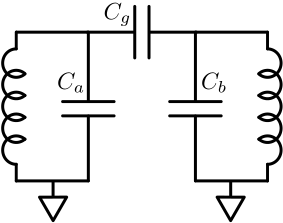
\includegraphics[width=6cm]{coupled_circuits_capacitive.pdf}
\par\end{centering}
\caption{Two circuits coupled through a capacitor $C_g$.}
\label{Fig:coupledCircuits_capacitive}
\end{figure}

The circuit shown in Fig.\,\ref{Fig:coupledCircuits_capacitive} has the following Lagrangian \begin{align}
\mathcal{L} = & \frac{1}{2}C_1\dot{\Phi}_1^2 + \frac{1}{2}C_2\dot{\Phi}_2^2 \nonumber \\
& + \frac{1}{2}C_g \left( \dot{\Phi}_1 - \dot{\Phi_2} \right)^2 \nonumber \\
& - \frac{1}{2L_1}\Phi_1^2 - \frac{1}{2L_2}\Phi_2^2 \, . \end{align}
The kinetic term can be rewritten as \begin{equation}
T = \frac{1}{2}
\left( \begin{array}{cc} \dot{\Phi}_1 & \dot{\Phi}_2 \end{array} \right)
\left( \begin{array}{cc} C_1' & -C_g \\ -C_g & C_2' \end{array} \right)
\left( \begin{array}{c} \dot{\Phi}_1 \\ \dot{\Phi}_2 \end{array} \right) \label{eq:kineticInFlux} \end{equation}
where $C_1' \equiv C_1+C_g$ and similarly for $C_2'$. The canonical momenta are \begin{eqnarray}
p_1 = \frac{dL}{d\dot{\Phi}_1} = C_1'\dot{\Phi}_1 - C_g\dot{\Phi}_2 \nonumber \\
p_2 = \frac{dL}{d\dot{\Phi}_2} = C_2'\dot{\Phi}_2 - C_g\dot{\Phi}_1 \end{eqnarray}
which can be written as \begin{equation}
\left( \begin{array}{c} p_1 \\ p_2 \end{array} \right) =
\left( \begin{array}{cc} C_1' & -C_g \\ -C_g & C_2' \end{array} \right)
\left( \begin{array}{c} \dot{\Phi}_1 \\ \dot{\Phi}_2 \end{array} \right) \end{equation}
Note the recurrence of the matrix from equation (\ref{eq:kineticInFlux}). Naming this matrix $M$ we can write \begin{eqnarray}
T &=& \frac{1}{2}
      \left( \begin{array}{cc} \dot{\Phi}_1&\dot{\Phi}_2 \end{array} \right)
      M
      \left( \begin{array}{c} \dot{\Phi}_1 \\ \dot{\Phi}_2 \end{array} \right) \label{eq:kineticWithM} \\
\left( \begin{array}{c} \dot{\Phi}_1 \\ \dot{\Phi}_2 \end{array} \right) &=& M^{-1} \left( \begin{array}{c} p_1 \\ p_2 \end{array} \right) \label{eq:fluxToMomenta} \end{eqnarray}
Substituting equation (\ref{eq:fluxToMomenta}) into (\ref{eq:kineticWithM}) and using the facts that matrix transposition commutes with matrix inversion and that $M$ is symmetric we get
\begin{equation}
T = \frac{1}{2} \left( \begin{array}{cc} p_1&p_2 \end{array} \right) M^{-1} \left( \begin{array}{c} p_1 \\ p_2 \end{array} \right) \, .
\end{equation}
The inverse of the 2x2 matrix $M$ is
\begin{align}
M^{-1} &= \frac{1}{C_1C_2 + C_g(C_1 + C_2)} \left( \begin{array}{cc} C_2' & C_g \\ C_g & C_1' \end{array} \right) \nonumber \\
&\equiv \left( \begin{array}{cc} 1/C_1'' & 1/C_g'' \\ 1/C_g'' & 1/C_2'' \end{array} \right) \, .
\end{align}
Finally, the kinetic term of the Langrangian is \begin{equation}
T = \frac{p_1^2}{2C_1''} + \frac{p_2^2}{2C_2''} + \frac{p_1p_2}{C_g''} \, . \label{eq:kineticInP}
\end{equation}

Let us now understand the quantities $C_1''$ and $C_2''$ in a simple way.
The capacitance to ground from the signal node of circuit 1 is \begin{eqnarray}
C_{1,\textrm{total}} &=& C_1||(C_g \textrm{ in series with } C_2) \nonumber \\
&=& C_1 + \frac{C_g C_2}{C_g+C_2} \nonumber \\
&=& \frac{C_1 C_2 + C_g(C_1+C_2)}{C_g+C_2} \nonumber \end{eqnarray}
which is exactly equal to our expression for $C_1''$.
Therefore we've found that \textbf{the effective capacitance associated with the the canonical charge is just the capacitance to ground of the conjugate flux's signal node}.

The quantities $p_1$ and $p_2$ have dimensions of charge so we will rename them $\tilde{Q}_1$ and $\tilde{Q}_2$.
The tildes remind us that they are not the usual single qubit charges.

The coupling term in the Hamiltonian, eq.\,(\ref{eq:kineticInP}), is \begin{equation}
H_g = \frac{ \tilde{Q}_1 \tilde{Q}_2} {C_g''}. \label{eq:sec:coupling:H_g} \end{equation}
We would like to re-express it in terms of Pauli operators.
If we use the (very good) approximation that the normal modes are harmonic we can rewrite the charge operators as \begin{equation}
\tilde{Q} = -i Q_{\textrm{zpf}} (a - a^{\dagger}) \, . \end{equation}
The parameter $Q_{\textrm{zpf}}$ is the rms zero point fluctuations in charge and is given by (see \citeinternaltype \citeinternalref{quantumOscillator}) \begin{equation}
Q_{\textrm{zpf}} = \sqrt{\frac{\hbar}{2Z}} = \sqrt{\frac{\hbar \omega C}{2}} \, . \end{equation}
Substitution of this expression for the $\tilde{Q}$ coordinates turns the coupling Hamiltonian into
\begin{align}
H_g &= \frac{Q_{1,\textrm{zpf}}Q_{2,\textrm{zpf}}}{C_g''}(-i)(a_1-a_1^{\dagger})(-i)(a_2-a_2^{\dagger}) \nonumber \\
&= \frac{\hbar}{2}\sqrt{\omega_1\omega_2 C_1'' C_2''}\frac{C_g}{C_1C_2 + C_g(C_1+C_2)}(\sigma_y \otimes \sigma_y) \nonumber \\
&= \frac{1}{2}\frac{C_g}{\sqrt{C_1' C_2'}} \hbar\sqrt{\omega_1\omega_2} (\sigma_y \otimes \sigma_y) \nonumber
\end{align}
where we have again used a two level approximation \mbox{$a - a^\dagger \rightarrow i \sigma_y$}.
We combine the prefactors into a parameter $g$ and write the Hamiltonian as \begin{equation}
H_g = g \left( \sigma_y \otimes \sigma_y \right) \end{equation}
where $g$, called the ``coupling strength'', is defined as \begin{equation}
g \equiv \frac{1}{2} \frac{C_g}{\sqrt{C_1' C_2'}} \hbar\sqrt{\omega_1\omega_2} \, . \end{equation}
Taking $C_1 \approx C_2$ and $\omega_1 \approx \omega_2$, then using $C = 1 / \omega Z_{LC}$ we find
\begin{equation}
g \propto Z_{LC} \, .
\end{equation}

\subsection{Summary - Simple derivation}

The energy in the coupling capacitor is
\begin{equation}
E_g = \frac{1}{2} C_g \left( V_1 - V_2 \right)^2 \, . \nonumber
\end{equation}
Keeping only the term which couples the qubits, we find \begin{equation}
E_g = -C_g V_1 V_2 = -C_g \frac{Q_1}{C_1} \frac{Q_2}{C_2} . \end{equation}
This matches Eq.\,(\ref{eq:sec:coupling:H_g}), up to the sign, in the practical limit $C_1,C_2 \gg C_g$.

\subsection{Inductive Coupling}

\begin{figure}
\begin{centering}
\includegraphics[width=6cm]{coupled_circuits_inductive.pdf}
\par\end{centering}
\caption{Two circuits coupled through a mutual inductance $M$.}
\label{Fig:coupledCircuits_inductive}
\end{figure}


Consider the circuit shown in Figure \ref{Fig:coupledCircuits_inductive}.
From Kirchoff's laws we find that the equations of motion for the system are
\begin{align}
\omega_1^2 Q_1 &= -\ddot{Q}_1 - \left(M/L_1\right) \ddot{Q}_2 \\
\omega_2^2 Q_2 &= -\ddot{Q}_2 - \left(M/L_2\right) \ddot{Q}_1
\end{align}
These equations of motion can be derived from the following Lagrangian
\begin{equation}
\mathcal{L} = \frac{Q_1^2}{2 C_1} + \frac{Q_2^2}{2 C_2}
- \frac{L_1}{2}\dot{Q}_1^2
- \frac{L_2}{2}\dot{Q}_2^2
- M \dot{Q}_1 \dot{Q}_2 \, . \label{eq:sec.coupling.subsec.inductiveCoupling:Lagrangian}
\end{equation}

In this Lagrangian the charges have appeared as the coordinate variables.
This is annoying because in all of our previous analysis we regarded the fluxes as the coordinates and the charges as the conjugate momenta.
To convert to using flux as the coordinate, we note that the $\dot{Q}$ are the loop currents, and we relate the currents to the fluxes using the definition of inductance and mutual inductance:
\begin{align}
\Phi_1 &= L_1 I_1 + M I_2 \\
\Phi_2 &= M I_1 + L_2 I_2 \, .
\end{align}
These equations are rewritten as a matrix equation
\begin{align}
\left( \begin{array}{c} \Phi_1 \\ \Phi_2 \end{array} \right) &=
\left[ \begin{array}{cc} L_1 & M \\ M & L_2 \end{array} \right]
\left( \begin{array}{c} I_1 \\ I_2 \end{array} \right) \\
\ket{\Phi} &= \mathbf{M} \ket{I} \label{eq:sec.coupling.subsec.inductiveCoupling:fluxToI} \, .
\end{align}
Next, using $\dot{Q}=I$, note that the dotted terms in Eq.\,(\ref{eq:sec.coupling.subsec.inductiveCoupling:Lagrangian}) can also be written as a matrix expression:
\begin{equation}
-\frac{1}{2} \bbraket{I}{\mathbf{M}}{I} \, .
\end{equation}
Therefore, by using Eq.\,(\ref{eq:sec.coupling.subsec.inductiveCoupling:fluxToI}) in Eq.\,(\ref{eq:sec.coupling.subsec.inductiveCoupling:Lagrangian}) we can rewrite the Lagrangian as
\begin{equation}
\mathcal{L} =
\frac{Q_1^2}{2 C_1} + \frac{Q_2^2}{2 C_2}
- \frac{1}{2} \bbraket{\Phi}{\mathbf{M}^{-1}}{\Phi} \, .
\end{equation}
To get a true Lagrangian we have to express the charges in terms of flux.
Using the definition of capacitance, $C = Q/V$, and noting that the \emph{total} flux through each inductor is the time integral of the voltage, we have
\begin{equation}
\frac{1}{2}\frac{Q^2}{C} = \frac{1}{2}C \dot{\Phi}^2 \, .
\end{equation}
Using this and expanding $\mathbf{M}^{-1}$ we finally arrive at
\begin{align}
\mathcal{L} &=
\frac{1}{2}C_1 \dot{\Phi}_1^2 + \frac{1}{2}C_2 \dot{\Phi}_2^2 \\
&- \left( \frac{1}{1 - M^2 / L_1L_2} \right)
\left( \frac{\Phi_1^2}{2L_1} + \frac{\Phi_2^2}{2L_2} \right) \\
&+ \left( \frac{1}{1 - M^2 / L_1 L_2} \right) \frac{M}{L_1 L_2} \Phi_1 \Phi_2 \, .
\end{align}
Thus we have reformulated the Lagrangian with the fluxes as the coordinates.

The conjugate momenta are
\begin{equation}
p = \frac{\partial \mathcal{L}}{\partial \dot{\Phi}} = C \dot{\Phi} = Q \, .
\end{equation}
The Hamiltonian is
\begin{align}
H &= \sum_i Q_i \dot{\Phi}_i - \mathcal{L} \\
&= \frac{Q_1^2}{2 C_1} + \frac{Q_2^2}{2 C_2} \\
&+ \left( \frac{1}{1 - M^2 / L_1L_2} \right)
\left( \frac{\Phi_1^2}{2L_1} + \frac{\Phi_2^2}{2L_2} \right) \\
&+ \left( \frac{1}{1 - M^2 / L_1 L_2} \right) \frac{M}{L_1 L_2} \Phi_1 \Phi_2 \, .
\end{align}


\section{Rotating Frame}

The driving and coupling Hamiltonians we have written down are not well suited for calculations because they do not commute with the intrinsic qubit Hamiltonian, which is typically proportional to either $\sigma_x$ or $\sigma_z$.
This non-commutativity is the mathematical manifestation of the physical fact that, in the lab frame, the qubit state processes about an axis in the Block sphere.
For this reason, it is much easier to reason in a frame that rotates about that axis at a frequency near or equal to the resonance frequency of the device, i.e. in a rotating frame.
In this section we show how to re-express the driving and coupling Hamiltonians in a rotating frame.

The single qubit Hamiltonian for single nearly harmonic qubits like the transmon is \begin{equation}
H_q/\hbar = -\frac{\omega_q}{2}\sigma_z \end{equation}
where $\omega_q = \omega_0 + \delta\omega$. Think of $\omega_0$ as an idle point frequency and $\delta \omega$ as a dynamic detuning.
The Schrodinger picture time evolution operator is $T=\exp \left[-i H/\hbar \right]$.
In order to remove the idle point precession of the qubit state, we take as the rotation operator \begin{equation}
R = T^{\dagger} = \exp \left[ -i \frac{\omega_0}{2} t \sigma_z \right], \end{equation}
eg. we rotate the frame by the idle frequency of the qubit.
We compute the remaining effective Hamiltonian $H'$ according to \citeinternalref{quantumMechanics} \begin{eqnarray}
H'/\hbar &=& i\dot{R}R^{\dagger} + R \frac{H_q}{\hbar} R \\
&=& i \left(-i \frac{\omega_0}{2} \right)\sigma_z RR^{\dagger} + R\frac{H_q}{\hbar}R^{\dagger} \\
&=& -\frac{\delta\omega}{2}\sigma_z. \end{eqnarray}
This is precisely the Hamiltonian of a qubit with frequency $\delta\omega$.
In other words, if we go into a frame rotating at the idle frequency of the qubit, what remains is just the qubit precession at the detuning frequency.
In particular if the frame rotates at the same frequency as the qubit the Hamiltonian becomes zero.

\subsection{Operators}

Since we are going to want to work in a frame in which the qubit intrinsic Hamiltonian is zero it will be useful to find the form of various operators in that frame.
We list here the transformation of the Pauli operators under a frame rotating about the z-axis at frequency $\omega_r$.
The rotation operator is $R=\exp \left[-i \frac{1}{2} \omega_r t \sigma_z \right]$ \citeinternalref{quantumMechanics} and the transformed Pauli operators are \begin{align}
R\sigma_xR^{\dagger} & = \cos(\omega_r t)\sigma_x + \sin(\omega_r t) \sigma_y \nonumber \\
R\sigma_yR^{\dagger} & = \cos(\omega_r t)\sigma_y - \sin(\omega_r t) \sigma_x \nonumber \\
R\sigma_zR^{\dagger} & = \sigma_z \nonumber \\
R\sigma_+R^{\dagger} & = e^{i\omega_r t}\sigma_+ \nonumber \\
R\sigma_-R^{\dagger} & = e^{-i\omega_r t}\sigma_- \, . \nonumber \end{align}

\subsection{Driving}

We now consider the driving Hamiltonian in the rotating frame.
From section \ref{sec:driving} we have the general driving Hamiltonian in the lab frame
\begin{equation}
H_d = h_d f(t) \sigma \, .
\end{equation}
For charge driving, we have $\sigma = \sigma_y$, $V_d(t) = V_d f(t)$, and $h_d = \bbraket{1}{Q}{0} V_d/(1 + C/C_d)$.
For flux driving, we have $\sigma = \sigma_x$, $I_d(t) = I_d f(t)$, and $h_d = (M/L) \bbraket{1}{\Phi}{0} I_d$.
We consider the flux case to for the sake of a specific example.
We use the rotation operator \begin{equation}
R = \exp \left[ -i \frac{\omega_r}{2} t \sigma_z \right] \end{equation}
to find the transformed driving Hamiltonian \begin{align}
RH_d R^{\dagger}/h_d
&= e^{-i \frac{\omega_r}{2} t \sigma_z} f(t)\sigma_x e^{i \frac{\omega_r}{2} t \sigma_z} \nonumber \\
&= f(t)\left[ \cos\left(\omega_r t\right)\sigma_x + \sin\left(\omega_r t\right)\sigma_y \right]. \label{eq:drivingH}
\end{align}
Now suppose $f(t)$ is a sinusoid with an envelope $e(t)$,
\begin{align}
& f(t)
= e(t)\cos \left( \omega_d t + \phi_d \right) \\
&= e(t) \left[ \cos \left( \phi_d \right) \cos \left( \omega_d t \right) - \sin \left( \phi_d \right) \sin \left( \omega_d t \right) \right] \\
&= e(t) \left[ I \cos\left(\omega_d t\right) + Q \sin \left(\omega_d t\right) \right] \label{eq:drivingFunctionIQ}
\end{align}
where $I \equiv \cos(\phi_d)$ and $Q \equiv - \sin(\phi_d)$.
Multiplying everything in Eq. (\ref{eq:drivingH}) together and throwing out the high frequency terms we get
\begin{align}
& RH_dR^{\dagger}/h_d \\
&= \frac{e(t)}{2} \left[ \cos(\delta\omega t + \phi_d)\sigma_x - \sin(\delta\omega t + \phi_d)\sigma_y \right] \\
&= \frac{e(t)}{2} \left[ e^{-i(\delta \omega t + \phi_d)} \sigma_+ + e^{i(\delta \omega t + \phi_d)} \sigma_- \right]
\end{align}
where $\delta\omega \equiv \omega_d - \omega_r$. In matrix form this reads
\begin{equation}
RH_dH^{\dagger}/h_d = \frac{e(t)}{2} \left( \begin{array}{cc} 0 & e^{i(\delta\omega t + \phi_d)} \\ e^{-i(\delta\omega t + \phi_d)} & 0 \end{array}\right) \, . \label{eq:drivingH_matrixForm}
\end{equation}
If the drive is on resonance with the frame, and therefore on resonance with the qubit, then we are left with
\begin{align}
RH_dR^{\dagger}/h_d
&= \frac{e(t)}{2}\left( \begin{array}{cc} 0 & e^{i\phi_d} \\ e^{-i\phi_d} & 0 \end{array}\right) \\
&= \frac{e(t)}{2} \left[ I \sigma_x + Q \sigma_y \right] .
\end{align}
This is a rotation about a time independent axis in the xy plane of the Bloch sphere.
If the rotating frame frequency is the same as the qubit frequency, then the qubit Hamiltonian is zero and our on-resonance drive leads to a purely latitudinal rotation on the Bloch sphere with the angle of the rotation axis in the xy plane given by $\phi$.
If the qubit frequency does not match the rotating frame then the qubit Hamiltonian has a residual $\sigma_z$ component and the the rotation axis will be out of the xy plane.

\subsubsection{$\pi$ pulse}

For a resonant drive with $\phi_d=0$ we have \begin{equation}
RH_dR^{\dagger} = -\frac{e(t)}{2}\frac{V_d \left| \bbraket{1}{Q}{0} \right|} {1 + C/C_d} \sigma_x. \end{equation}
The evolution of the qubit under this drive is given by the unitary operator \begin{equation}
U(t) = \exp \left[ i \left( \frac{1}{2 \hbar} \frac{V_d \left| \bbraket{1}{Q}{0} \right|} {1 + C/C_d} \int dt \, e(t) \right) \sigma_x \right]. \end{equation}
This results in a pi pulse when $U(t)=\sigma_x$. Since \begin{equation}
\exp \left[ i \alpha \sigma_x \right] = \cos(\alpha)\textrm{I} + i \sin(\alpha)\sigma_x \end{equation}
we see that the pi pulse occurs when \begin{equation}
\frac{1}{2\hbar} \frac{V_d \left| \bbraket{1}{Q}{0} \right|} {1 + C/C_d} \int e(t) dt = \frac{\pi}{2} \, . \end{equation}
This relation is used to determine the appropriate drive capacitance $C_d$ when designing a device.
The accessible values of $V_0$ are determined by the dynamic range of available pulse generators, the level of attenuation needed to remove noise from the drive lines.
The value of $C_d$, is then chosen to be large enough that a $\pi$-pulse can be done in an acceptably short time while preserving the qubit coherence as discussed above.
The value of $Q_{\textrm{zpf}}$ is determined by the type of qubit.

\subsubsection{Programming for experiment}

Now that we know what the driving Hamiltonian looks like in the rotating frame we can investigate how to program our IF inputs to the IQ mixer to acheive a rotation on the Bloch sphere.
From \citeinternalref{IQMixer} we know that an input IQ signal $e(t)\exp\left[i\omega t + \phi\right]$ produces an RF signal $ e(t)\cos\left[(\omega_c+\omega)t + \phi \right]$, where $\omega_c$ is the carrier frequency. Using trig identities we can rewrite this RF signal as \begin{equation}
e(t) \left[ I\cos(\left[\omega_c+\omega\right] t) + Q\sin(\left[\omega_c+\omega\right]t)\right] \nonumber \end{equation}
where $I=\cos(\phi)$ and $Q=-\sin(\phi)$.
This exactly matches the form we assumed for $f(t)$ in eq. (\ref{eq:drivingFunctionIQ}) if we take $\omega_c + \omega = \omega_d$.
Therefore if we choose $\omega$ such that $\omega + \omega_c = \omega_q$ and work in the rotating frame of the qubit, the driving Hamiltonian is \begin{equation}
H_d/h_d = \frac{e(t)}{2}\left[I\sigma_x + Q\sigma_y\right]. \end{equation}
In practice we don't want to have to remember to account for the carrier frequency when programming a pulse so we define a mix function which multiplies our complex signal by $\exp\left[i(\omega_{q} - \omega_c)\right]$.
That way if we program a signal $\exp\left[i\phi\right]$ the driving Hamiltonian in the frame of the qubit is produced in the following steps \begin{align}
&\textrm{program} e(t) e^{i\phi} \nonumber \\
&\stackrel{\textrm{mix function}}{\longrightarrow} e(t) e^{i([\omega_q-\omega_c]t + \phi)} \nonumber \\
&\stackrel{\textrm{physical mixer}}{\longrightarrow} \Re \left[ e(t) e^{i(\omega_q t + \phi)} \right] = e(t) \cos\left(\omega_q t + \phi \right) \nonumber \\
&\stackrel{\textrm{Hamiltonian}}{\longrightarrow} \frac{e(t)}{2}\left[ I \sigma_x + Q \sigma_y \right]. \nonumber
\end{align}
Thus our choice of angle $\phi$ directly maps to the angle of the rotation on the Bloch sphere.

\subsection{Coupling}

We found that the coupling Hamiltonian in the Schro-dinger picture is \begin{equation}
H_g = g \left( \sigma_y \otimes \sigma_y \right) \end{equation}
which can be expanded as \begin{eqnarray}
H_g &=& -g (\sigma^+ - \sigma^-) \otimes (\sigma^+ - \sigma^-) \nonumber \\
&=& g \left(-\sigma^+ \sigma^+ - \sigma^- \sigma^- + \sigma^+ \sigma^- + \sigma^- \sigma^+ \right). \end{eqnarray}
Rotating the qubits' frames at $\omega_{r1}$ and $\omega_{r2}$ respectively and throwing away high frequency terms we get \begin{equation}
H_g = g \left( e^{i \delta\omega_{r12} t} \sigma^+ \sigma^- + e^{-i \delta\omega_{r12} t} \sigma^- \sigma^+ \right) \end{equation}
where $\delta\omega_{r12}\equiv \omega_{r1} - \omega_{r2}$.
If both frames rotate at the same frequency the interaction simplifies to \begin{equation}
H_g = g \left( \sigma^+ \sigma^- + \sigma^- \sigma^+ \right). \end{equation}
The matrix form, with basis states \begin{equation}
\left[ \ket{00}, \ket{01}, \ket{10}, \ket{11} \right] \nonumber \end{equation}
(ie the states defined by Kronecker product) is \begin{equation}
H_g = g \left[ \begin{array}{cccc} 0 & 0 & 0 & 0 \\ 0 & 0 & 1 & 0 \\ 0 & 1 & 0 & 0 \\ 0 & 0 & 0 & 0 \end{array} \right]. \end{equation}
This shows that direct on-resonance capacitive coupling produces a swap interaction in which excitations oscillate between the two coupled qubits.
This is an entangling interaction.

%\subsubsection{Do LO phases matter?}

%We can now answer the question of whether we need to keep LO oscillator phases stable across multiple repetitions of a multiple qubit experiment. Consider an experiment in which we have to capacitively coupled qubits and an adjustable coupling $g(t)$. We put the qubits on resonance and rotate each qubit's frame at  qubit frequency. As previously explained in this doubly rotating frame the intrinsic qubit Hamiltonians are zero and the coupling Hamiltonian is $g(t)\left( \sigma^+ \sigma^- + \sigma^- \sigma^+ \right)$. We now subject the system to one of the following control sequences \begin{eqnarray}
%X_{\pi/2}^{(1)} \rightarrow & \textrm{turn g on for a swap} & \rightarrow X_{\pi/2}^{(2)} \rightarrow \textrm{measure qubit 2} \nonumber \\
%X_{-\pi/2}^{(1)} \rightarrow & \textrm{turn g on for a swap} & \rightarrow X_{\pi/2}^{(2)} \rightarrow \textrm{Measure qubit 2} \nonumber \end{eqnarray}
%In the first case we will measure $\ket{1}$ but in the second we will measure $\ket{0}$.  As explained in the section on driving in the rotating frame, the difference in the leading $X$ pulses is just a difference in the phase of the drive voltage. This phase could come from an intentional choice of our I and Q signals, or from a change in the LO phase. Therefore, in general LO phase drift will mess up experiments. This could be verified by the pulse sequence we've considered here, measuring ramsey fringes on qubit 2 as a function of the drive phase on qubit 1.


\bibliographystyle{plain}
\bibliography{../Bibliography/references_main,../Bibliography/references_local}

\end{document}
